%% Fall 2013 MDM Homework One
\documentclass[12pt,letterpaper]{article}

\usepackage[utf8]{inputenc}
\usepackage[T1]{fontenc}
\usepackage{amsmath}
\usepackage{amsfonts}
\usepackage{amssymb}
\usepackage{amsthm}
\usepackage[left=2cm,right=2cm,top=2cm,bottom=2cm,headheight=22pt]{geometry}
\usepackage{fancyhdr}
\usepackage{setspace}
\usepackage{lastpage}
\usepackage{url}
\usepackage{graphicx}

\theoremstyle{definition}
\newtheorem{task}{Task}

\begin{document}

%other parameters
\setlength{\parskip}{1ex plus 0.5ex minus 0.2ex}
\setlength{\parindent}{0pt}

%header and footer parameters
\pagestyle{fancy}
\lhead{Math 1100}
\chead{Weekly Homework}
\rhead{Due: Friday, February 5 by 3pm}
\lfoot{} 
\cfoot{\emph{Prof. Hitchman}} 
\rfoot{} 

\begin{center}
{
\Large
\textbf{Graphs: Assignment \#4}
}
\end{center}

Your paper should have the following information on it.
\begin{itemize}
\item Your name
\item Your student ID number 
\item Which section you are in: 02 MWF, or 04 TTh
\end{itemize}


\subsection*{Specifications for Grading}

To earn a passing mark, your assignment must:
\begin{itemize}
\item be typed, and at least one page and no more than two pages in length. Diagrams may be hand drawn.
\item address the tasks and questions below.
\item explain your ideas in complete sentences. Use paragraphs to organize your thoughts.
\item conform to reasonable standards for grammar, spelling, and usage of the English language with minimal errors. (You may consider seeking help on writing from the Writing Center in the Academic Learning Center. http://www.uni.edu/unialc/writing-center)
\item be turned in by 3pm on Friday, January 22.
\end{itemize}



\subsection*{What to do}

\begin{task}
The graph below has its vertices labeled in alphabetical order. Use this ordering in the algorithm for finding an
Eulerian cycle. Your end result should be an ordered list of vertices which describe the path you follow along 
the Eulerian cycle. Write down this list of vertices.
\begin{figure}[h]
\centering
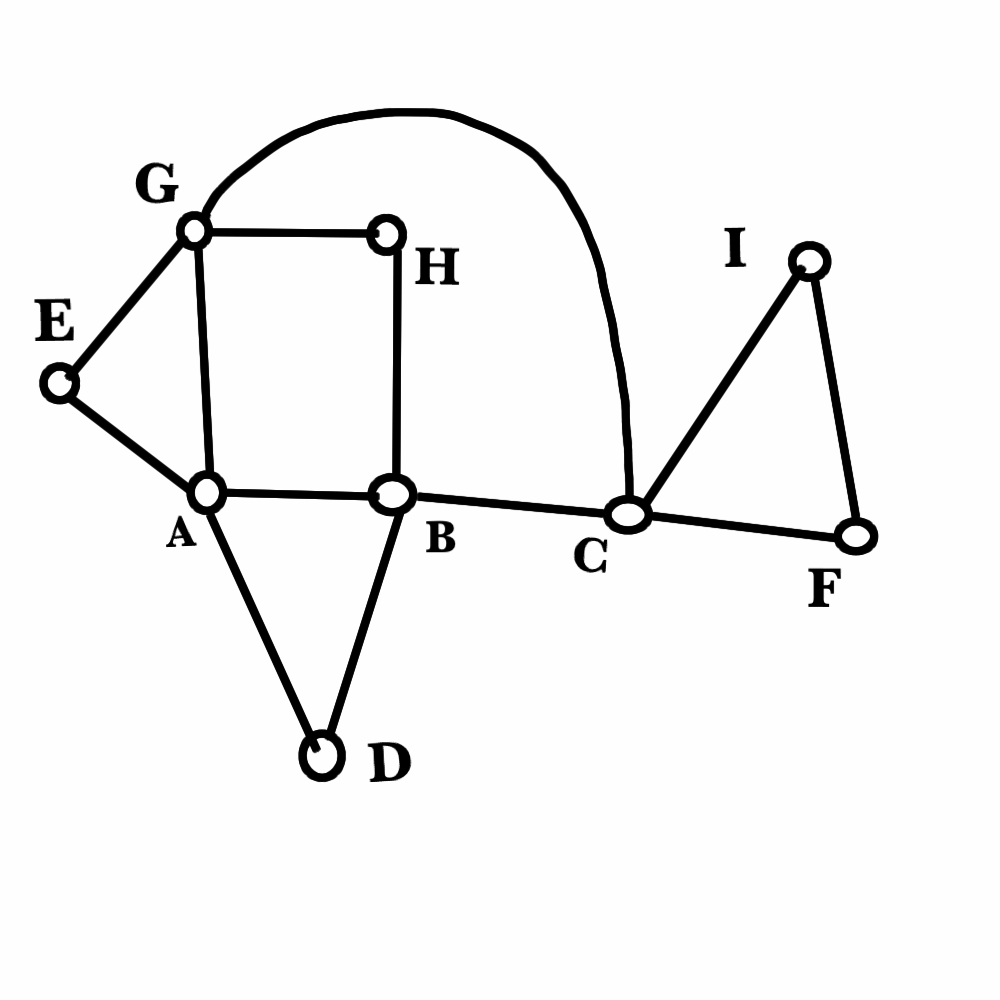
\includegraphics[width=.4\textwidth]{images/eulerian-hwk.png}
\label{A funny Eulerian graph}
\end{figure}
\end{task}

\begin{task}
Make an example of a graph which \textbf{does not} have a 4-coloring. Draw your graph and write an explanation of 
how you know your example has the property required.
\end{task}

\begin{task}
Figure out the chromatic number for the graph below. Write a detailed explanation for why you know your answer
is the correct one.
\begin{figure}[h]
\centering
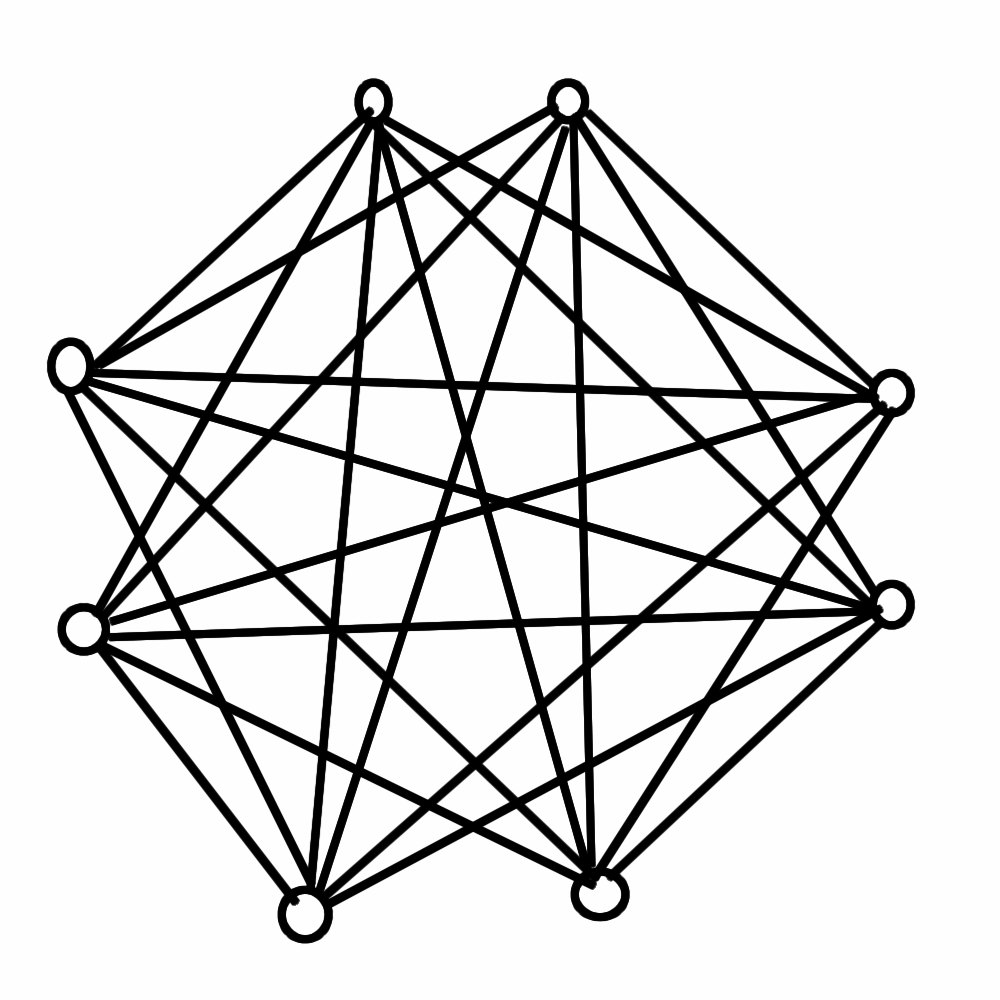
\includegraphics[width=.7\textwidth]{images/K2222.png}
\label{A graph with a lot of edges, but only eight vertices}
\end{figure}

\end{task}

\end{document}


















